%插入样式内容
\documentclass[12pt]{article}
%%---------------------------------------------------------------------
% packages
% geometry
\usepackage{color}
\usepackage{geometry}
% font
\usepackage{fontspec}
\defaultfontfeatures{Mapping=tex-text}  %%如果没有它,会有一些 tex 特殊字符无法正常使用,比如连字符。
\usepackage{xunicode,xltxtra}
\usepackage[BoldFont,SlantFont,CJKnumber,CJKchecksingle]{xeCJK}  % \CJKnumber{12345}: 一万二千三百四十五
\usepackage{CJKfntef}  %%实现对汉字加点、下划线等。
\usepackage{pifont}  % \ding{}
% math
\usepackage{amsmath,amsfonts,amssymb}
% color
\usepackage{color}
\usepackage{xcolor}
\definecolor{EYE}{RGB}{199,237,204}
\definecolor{FLY}{RGB}{128,0,128}
\definecolor{ZHY}{RGB}{139,0,255}
% graphics
\usepackage[americaninductors,europeanresistors]{circuitikz}
\usepackage{tikz}
\usetikzlibrary{positioning,arrows,shadows,shapes,calc,mindmap,trees,backgrounds}  % placements=positioning
\usepackage{graphicx}  % \includegraphics[]{}
\usepackage{subfigure}  %%图形或表格并排排列
% table
\usepackage{colortbl,dcolumn}  %% 彩色表格
\usepackage{multirow}
\usepackage{multicol}
\usepackage{booktabs}
% code
\usepackage{fancyvrb}
\usepackage{listings}
% title
\usepackage{titlesec}
% head/foot
\usepackage{fancyhdr}
% ref
\usepackage{hyperref}
% pagecolor
\usepackage[pagecolor={EYE}]{pagecolor}
% tightly-packed lists
\usepackage{mdwlist}

\usepackage{styles/iplouccfg}
\usepackage{styles/zhfontcfg}
\usepackage{styles/iplouclistings}
\usepackage{listings} 
\usepackage{hyperref}
\usepackage{color,framed}
%\usepackage{styles/pythonhighlight}
%\usepackage{graphicx}
%%---------------------------------------------------------------------
% settings
% geometry
\geometry{left=2cm,right=1cm,top=2cm,bottom=2cm}  %设置 上、左、下、右 页边距
\linespread{1.5} %行间距
% font
\setCJKmainfont{Adobe Kaiti Std}
%\setmainfont[BoldFont=Adobe Garamond Pro Bold]{Apple Garamond}  % 英文字体
%\setmainfont[BoldFont=Adobe Garamond Pro Bold,SmallCapsFont=Apple Garamond,SmallCapsFeatures={Scale=0.7}]{Apple Garamond}  %%苹果字体没有SmallCaps
\setCJKmonofont{Adobe Fangsong Std}
% graphics
\graphicspath{{figures/}}
\tikzset{
    % Define standard arrow tip
    >=stealth',
    % Define style for boxes
    punkt/.style={
           rectangle,
           rounded corners,
           draw=black, very thick,
           text width=6.5em,
           minimum height=2em,
           text centered},
    % Define arrow style
    pil/.style={
           ->,
           thick,
           shorten <=2pt,
           shorten >=2pt,},
    % Define style for FlyZhyBall
    FlyZhyBall/.style={
      circle,
      minimum size=6mm,
      inner sep=0.5pt,
      ball color=red!50!blue,
      text=white,},
    % Define style for FlyZhyRectangle
    FlyZhyRectangle/.style={
      rectangle,
      rounded corners,
      minimum size=6mm,
      ball color=red!50!blue,
      text=white,},
    % Define style for zhyfly
    zhyfly/.style={
      rectangle,
      rounded corners,
      minimum size=6mm,
      ball color=red!25!blue,
      text=white,},
    % Define style for new rectangle
    nrectangle/.style={
      rectangle,
      draw=#1!50,
      fill=#1!20,
      minimum size=5mm,
      inner sep=0.1pt,}
}
\ctikzset{
  bipoles/length=.8cm
}
% code
\lstnewenvironment{VHDLcode}[1][]{%
  \lstset{
    basicstyle=\footnotesize\ttfamily\color{black},%
    columns=flexible,%
    framexleftmargin=.7mm,frame=shadowbox,%
    rulesepcolor=\color{blue},%
%    frame=single,%
    backgroundcolor=\color{yellow!20},%
    xleftmargin=1.2\fboxsep,%
    xrightmargin=.7\fboxsep,%
    numbers=left,numberstyle=\tiny\color{blue},%
    numberblanklines=false,numbersep=7pt,%
    language=VHDL%
    }\lstset{#1}}{}
\lstnewenvironment{VHDLmiddle}[1][]{%
  \lstset{
    basicstyle=\scriptsize\ttfamily\color{black},%
    columns=flexible,%
    framexleftmargin=.7mm,frame=shadowbox,%
    rulesepcolor=\color{blue},%
%    frame=single,%
    backgroundcolor=\color{yellow!20},%
    xleftmargin=1.2\fboxsep,%
    xrightmargin=.7\fboxsep,%
    numbers=left,numberstyle=\tiny\color{blue},%
    numberblanklines=false,numbersep=7pt,%
    language=VHDL%
    }\lstset{#1}}{}
\lstnewenvironment{VHDLsmall}[1][]{%
  \lstset{
    basicstyle=\tiny\ttfamily\color{black},%
    columns=flexible,%
    framexleftmargin=.7mm,frame=shadowbox,%
    rulesepcolor=\color{blue},%
%    frame=single,%
    backgroundcolor=\color{yellow!20},%
    xleftmargin=1.2\fboxsep,%
    xrightmargin=.7\fboxsep,%
    numbers=left,numberstyle=\tiny\color{blue},%
    numberblanklines=false,numbersep=7pt,%
    language=VHDL%
    }\lstset{#1}}{}
% pdf
\hypersetup{%pdfpagemode=FullScreen,%
            pdfauthor={Haiyong Zheng},%
            pdftitle={Title},%
            CJKbookmarks=true,%
            bookmarksnumbered=true,%
            bookmarksopen=false,%
            plainpages=false,%
            colorlinks=true,%
            citecolor=green,%
            filecolor=magenta,%
            linkcolor=cyan,%red(default)
            urlcolor=cyan}
% section
%http://tex.stackexchange.com/questions/34288/how-to-place-a-shaded-box-around-a-section-label-and-name
\newcommand\titlebar{%
\tikz[baseline,trim left=3.1cm,trim right=3cm] {
    \fill [cyan!25] (2.5cm,-1ex) rectangle (\textwidth+3.1cm,2.5ex);
    \node [
        fill=cyan!60!white,
        anchor= base east,
        rounded rectangle,
        minimum height=3.5ex] at (3cm,0) {
        \textbf{\thesection.}
    };
}%
}
\titleformat{\section}{\Large\bf\color{blue}}{\titlebar}{0.1cm}{}
% head/foot
\setlength{\headheight}{15pt}
\pagestyle{fancy}
\fancyhf{}

\chead{\color{black!50!green}Cifar10 And MNIST}

%\lfoot{\color{blue!50!green}Dai Jialun}
\cfoot{\color{blue!50!green}\href{http://vision.ouc.edu.cn/~zhenghaiyong}{CVBIOUC}}
\rfoot{\color{blue!50!green}$\cdot$\ \thepage\ $\cdot$}
\renewcommand{\headrulewidth}{0.4pt}
\renewcommand{\footrulewidth}{0.4pt}


%%---------------------------------------------------------------------
\begin{document}
%%---------------------------------------------------------------------
%%---------------------------------------------------------------------
% \titlepage
\title{\vspace{-2em} 浮游动物识别分类——深度学习\\
\normalsize{}}
\author{Dai Jialun \hspace{0.25in} Wu Bin}
\date{\vspace{-0.7em} \today \vspace{-0.7em}}
%%---------------------------------------------------------------------
\maketitle\thispagestyle{fancy}
%%---------------------------------------------------------------------
\maketitle
%\tableofcontents 
\section{问题}
深度学习使用的数据库基本都是ImageNet,因此使用ImageNet与ZooScan的训练样本进行比较。
\begin{description}
\item[小数据] ZooScan的训练样本有13类(包含负样本),总共有9460张图片。ImageNet的ILSVRC 2013的训练样本有200类,总共395909张图片。
\item[分类] 将浮游动物分为不同种类,且种类数目较少,只有10种。
\item[数据的标注] ZooScan的训练图像中只有单个物体,即single-label,且背景为空白。ImageNet的训练图像基本都用多个不同物体的标注,即multiple-label。
\end{description}
\begin{figure}[!ht]
  \centering 
  \subfigure[]{ 
  %  \label{fig: } %% label for first subfigure 
    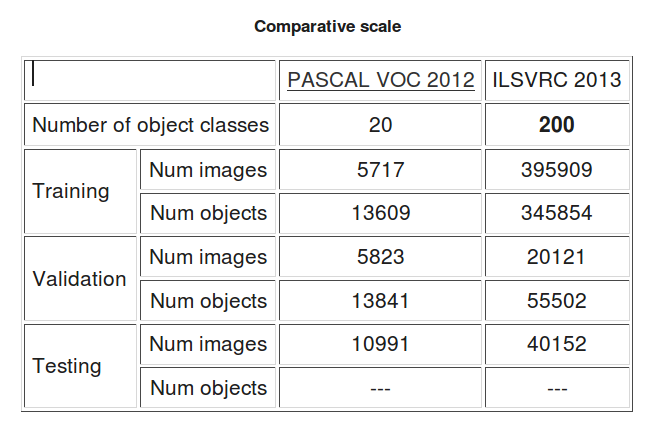
\includegraphics[width=0.32\textwidth]{ILSVRC}} 
  \subfigure[]{ 
  %  \label{fig: result1: b} %% label for second subfigure 
    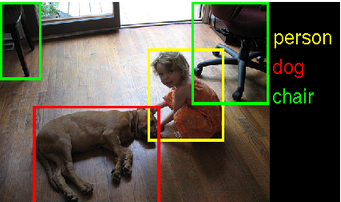
\includegraphics[width=0.35\textwidth]{ILSVRC2013}} 
  \caption{ILSVRC 2013}
%  \label{fig: } %% label for entire figure 
\end{figure}

\begin{figure}[!ht]
  \centering 
  \subfigure[]{ 
  %  \label{fig: } %% label for first subfigure 
    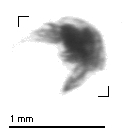
\includegraphics[width=0.185\textwidth]{zooplankton1}} 
  \subfigure[]{ 
 %   \label{fig: result1: b} %% label for second subfigure 
    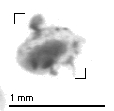
\includegraphics[width=0.2\textwidth]{zooplankton2}} 
  \caption{Zooplankton}
%  \label{fig: } %% label for entire figure 
\end{figure}


\section{可用方案}
\subsection{开源软件}
\begin{description}
\item[Caffe] Caffe是一个清晰而高效的深度学习框架,由表达式、速度和模块化组成,其作者是博士毕业于UC Berkeley的贾扬清。它具有有开放性架构、扩展代码、速度与社区化的优点。Caffe是纯粹的C++/CUDA架构,支持命令行、Python和MATLAB接口,而且可以在CPU和GPU直接无缝切换。

\item[cxxnet] 一个机器学习项目,其具有轻量而齐全的框架、强大统一的并行计算接口和易于扩展的代码结构。cxxnet平衡了python为主的编程效率和以c++为核心的为代表的追逐性能,使得我们在不损失效率的前提下可以通过模板编程技术允许开发者编写和matlab/numpy类似的代码,并且在编译时自动展开成优化的kernel。另外一些特性:CuDNN的支持、及时更新的最新技术、Caffe模型转换和方便的语言接口。

\item[Cuda-convnet] Cuda-convnet基于C++/CUDA编写,采用反向传播算法的深度卷积神经网络实现。Cuda-convnet 是 Alex Krizhevsky 公开的一套CNN代码,运行于Linux系统上,使用GPU做运算;2014年发布的版本可以支持多GPU上的数据并行和模型并行训练。(据说Alex的这套代码还是不太友好,按理说应该给出一个IO的标准,供后来人测试其他数据集的。)

\item[Theano] 提供了在深度学习数学计算方面的Python库,让你可以有效定义、优化和评价包含多维数组的数学公式。它整合了NumPy矩阵计算库、可以运行在GPU上、提供良好的算法上的扩展、在优化方面进行加速和稳定与动态C代码的生成等。

\item[OverFeat] 由纽约大学CILVR实验室开发的基于卷积神经网络系统,主要应用场景为图像识别和图像特征提取。主要使用C++编写的库来运行OverFeat卷积网络,可用数据增强来实现提高分类结果。

\item[Torch7] 一个为机器学习算法提供广泛支持的科学计算框架,其中的神经网络工具包(Package)实现了均方标准差代价函数、非线性激活函数和梯度下降训练神经网络的算法等基础模块,可以方便地配置出目标多层神经网络开展训练实验。
\end{description}

\subsection{网络模型}
在图像识别与分类上,主要使用卷积神经网络(Convolutional Neural Network, CNN)的网络模型来实现的。
\begin{description}
\item [AlexNet] AlexNet\cite{krizhevsky2012imagenet}是Hinton与其学生为了回应别人对于deep learning的质疑而将deep learning用于ImageNet的ILSVRC 2012上,结果优于当时最优的水平。该模型训练了一个深度卷积神经网络来完成分类和检测任务。AlexNet包含5层卷积层和3层全连接层。
\begin{figure}[!ht]
\centering
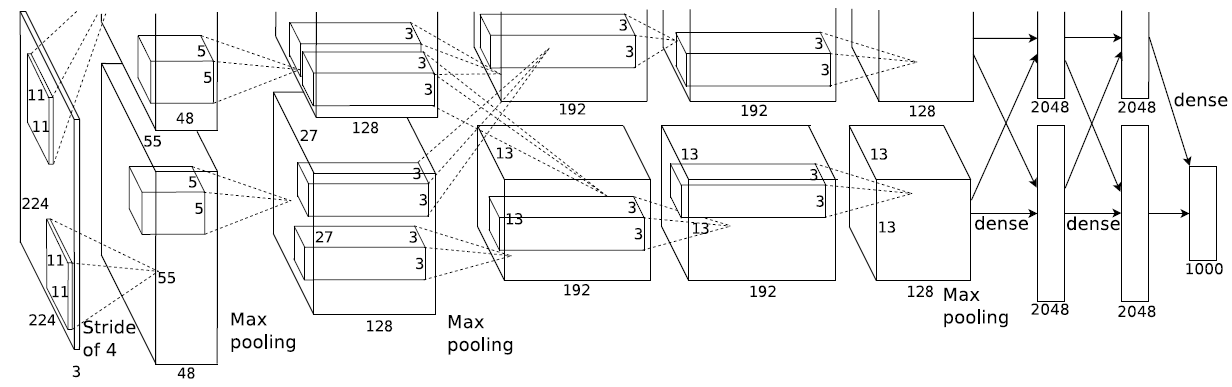
\includegraphics[width=0.6\textwidth]{AlexNet}
\caption{AlexNet}
%\label{fig:framework}
\end{figure}


\item[OverFeat] OverFeat\cite{sermanet2013overfeat}%\footnote{OverFeat: Integrated Recognition, Localization and Detection using Convolutional Networks}
由CILVR Lab,New York University开发的,基于卷积网络的图像识别和特征提取系统。
OverFeat的选举网络是由ImageNet 1K数据集训练的,参加了ILSVRC 2013分类、定位与检测竞赛。在Overfeat主要展示了多尺度和扫描窗口可以有效应用在卷积网络上。而且,不同的任务可以通过一个共享的学习网络来实现。
\begin{figure}[!ht]
\centering
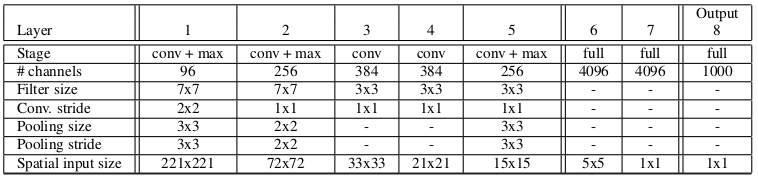
\includegraphics[width=0.65\textwidth]{overfeat}
\caption{overfeat}
%\label{fig:framework}
\end{figure}

\item[NIN] NIN(Network In Network)\cite{Lin:2013aa}是Learn­ing and Vi­sion Re­search Group,Na­tion­al Uni­ver­si­ty of Sin­ga­pore所使用的深度学习框架。他们团队通过在深度网络中建立更复杂的微型神经网络来提取数据。NIN网络包含了三个多元卷积层和一个全局平局pooling层。另外,他们团队提出``adaptive non-parametric rectification''方法来提高准确率。 
\begin{figure}[!ht]
\centering
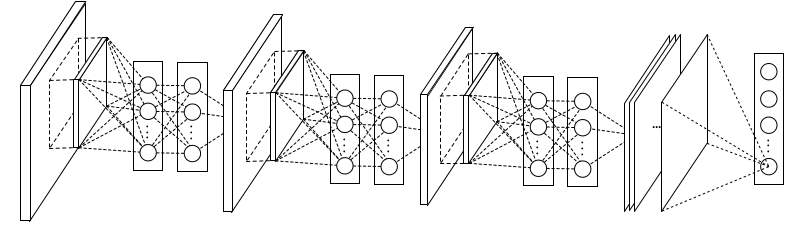
\includegraphics[width=0.55\textwidth]{NIN}
\caption{NIN}
%\label{fig:framework}
\end{figure}

\item[GoogLeNet] GoogLeNet\cite{simonyan2014very}是Google团队在ILSVRC 2014上,使用的深度学习网络模型,来完成分类和检测的任务。在GoogLeNet模型中,提出了Inception模型,即采用不同尺度的卷积核来处理问题。另外,该网络最大的特点就是提升了计算资源的利用率,即在网络所需计算不变的前提下,提升了网络的宽度和深度。最后,使用了基于Hebbian Principle和多尺寸处理来提高准确率。GoogLeNet包含pooling层在内,总共是27层的模型。
\begin{figure}[!ht]
\centering
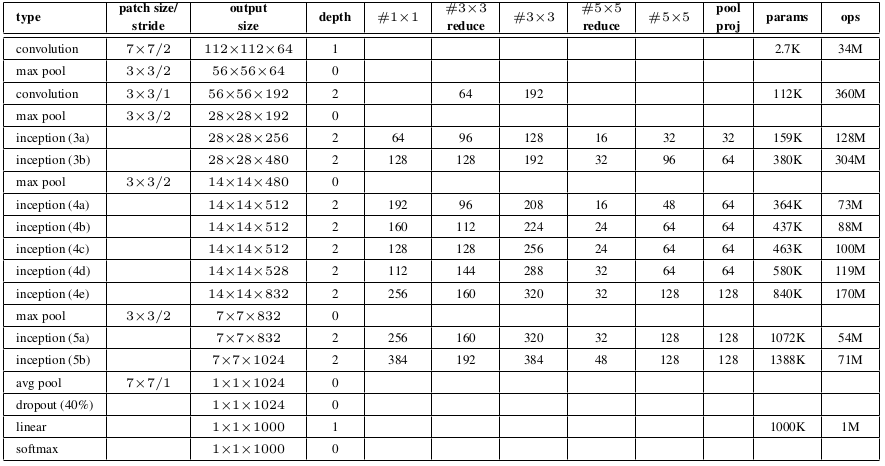
\includegraphics[width=0.65\textwidth]{googlenet}
\caption{GoogLeNet}
%\label{fig:framework}
\end{figure}
\item[ConvNet] ConvNet\cite{szegedy2014going}是Visual Geometry Group在ILSVRC 2014上,使用的深度学习网络模型。ConvNet与AlexNet的网络模型很相似,同为5组卷积层,3个全连接层。在ConvNet中,前5组的卷积层各有不同配置,即模型中有A$\sim$E,卷积层数从8到16递增。%,但最后通过加深卷积层数也到达提神准确率的瓶颈。
\begin{figure}[!ht]
\centering
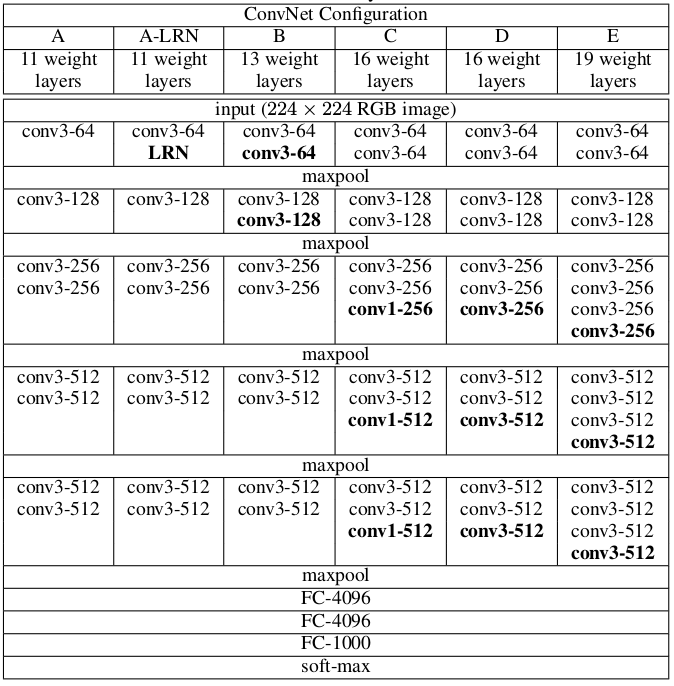
\includegraphics[width=0.42\textwidth]{vggnet2}
\caption{VGGNet}
%\label{fig:framework}
\end{figure}

\item[PCANet] PCANet是一个基于CNN的简化Deep Learning模型。经典的CNN存在的问题是参数训练时间过长且需要特别的调参技巧。PCANet模型是一种训练过程简单,且能适应不同任务、不同数据类型的网络模型。卷积核是直接通过PCA计算得到的,而不是像CNN一样通过反馈迭代得到的。
\begin{figure}[!ht]
\centering
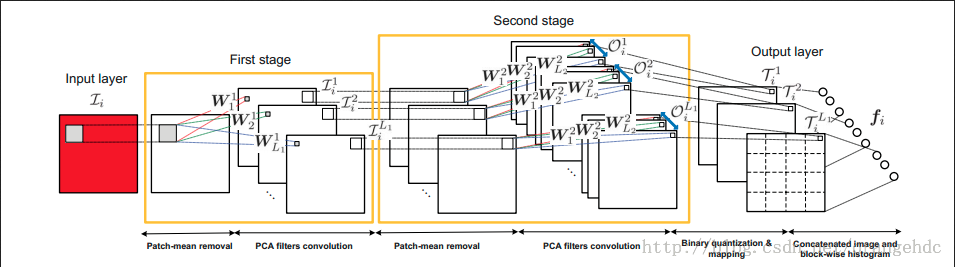
\includegraphics[width=0.65\textwidth]{PCANet}
\caption{PCANet}
%\label{fig:framework}
\end{figure}

\item[Deep Fisher Net] Deep Fisher Net\cite{simonyan2013deep}是Visual Geometry Group,University of Oxford在ILSVRC 2013分类上使用的模型,结合了两种深度框架:the deep Fisher vector network 和 the deep convolutional network。
\begin{figure}[!ht]
\centering
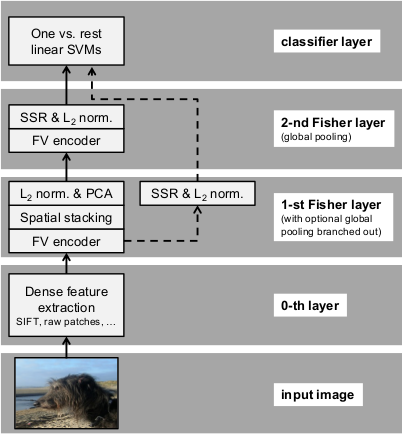
\includegraphics[width=0.3\textwidth]{vggnet1}
\caption{Deep Fisher Net}
%\label{fig:framework}
\end{figure}

\end{description}

\section{优化技巧}
\subsection{Dropout}
Dropout是指在模型训练时随机让网络某些隐含层节点的权重不工作,不工作的那些节点可以暂时认为不是网络结构的一部分,但是它的权重得保留下来,只是暂时不更新而已,因为下次样本输入时可能会工作。

应用在全连接层,是一种引入噪声机制,避免过拟合的有效正规化方法。适用于样本数目数 $\ll$ 模型参数。对于每一个隐层的output,以50\%的概略将它们设置为0,不再对与forward或backward过程起作用,即迫使每个神经元不依赖某些特定神经元独立工作,从而学到更有用的特征。
\begin{figure}[!ht]
  \centering 
  \subfigure[]{ 
 %   \label{fig: } %% label for first subfigure 
    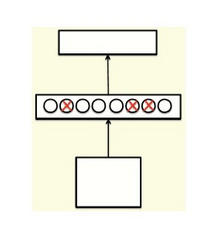
\includegraphics[width=0.25\textwidth]{dropout}} 
  \subfigure[]{ 
 %   \label{fig: result1: b} %% label for second subfigure 
    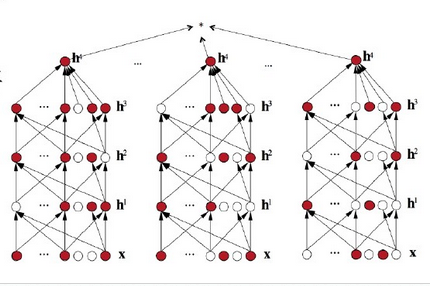
\includegraphics[width=0.4\textwidth]{dropout1}} 
  \caption{ILSVRC 2013}
 % \label{fig: } %% label for entire figure 
\end{figure}


\subsection{Pooling}
基于图像的局部信息与全局信息,可认为一个图像区域有用的特征极有可能在另一个区域同样适用。而且为了描述大的图像,可以对不同位置的特征进行聚合统计。

在卷积神经网络中,经常在卷积层后加入池化操作(pooling),通过池化来降低卷积层输出的特征向量维数,即用更高层的抽象表示图像特征,实现信息的融合。常见的池化操作分为为平均池化mean pooling和最大池化max pooling。
\begin{figure}[!ht]
\centering
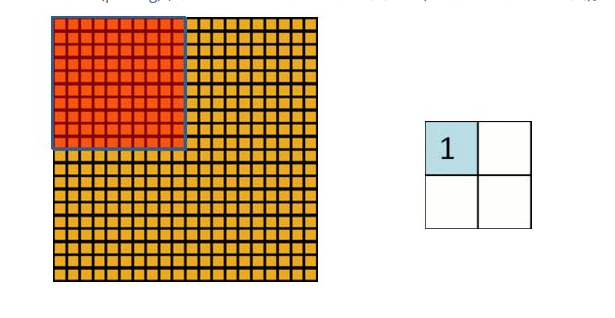
\includegraphics[width=0.5\textwidth]{pooling}
\caption{Pooling}
%\label{fig:framework}
\end{figure}

\subsection{PCA}
PCA(Principal Component Analysis),主成分分析,不仅仅是对高维数据进行降维,更重要的是经过降维去除了噪声,发现了数据中的模式。PCA把原先的n个特征用数目更少的m个特征取代,新特征是旧特征的线性组合,这些线性组合最大化样本方差,尽量使新的m个特征互不相关。从旧特征到新特征的映射捕获数据中的固有变异性。对每个RGB图像进行一个PCA变换,完成了去噪功能与保证图像多样性。可认为,加入了一个随机尺度因子,每一轮重新生成一个尺度因子,保证了同一副图像中在显著特征上有一定范围的变换,降低overfitting。

PCA过程:
\begin{enumerate}
\item 特征中心化。即每一维的数据都减去该维的均值。
\item 计算数据的协方差矩阵
\item 计算协方差矩阵C的特征值和特征向量
\item 选取大的特征值对应的特征向量,得到新的数据集。
\end{enumerate}

\subsection{Image transformation}
通过对于图像的变换实现了对于数据集合的扩大,在位置的维度上丰富了训练数据。降低了overfitting和网络结构设计的复杂程度。

\subsection{LPN}
Local Response Normalization,局部响应归一化。完成``临近抑制''操作,对局部输入区域进行归一化。在通道间归一化模式中,局部区域范围在相邻通道间,没有空间扩展。在通道内归一化模式中,局部区域在空间上扩展,只针对独立通道进行。

\subsection{Pre-training}
``逐层初始化''(Layer-wise Pre-training)。采用的逐层贪婪训练方法来训练网络的参数,即先训练网络的第一个隐含层,解得到较好的值作为第一层的初始参数。然后接着训练第二层,第三层。最后用这些训练好的网络参数值作为整体网络参数的初始值。前几层的网络层次基本都用无监督的方法容易获得,只有最后一个输出层需要有监督的数据。
\begin{figure}[!ht]
\centering
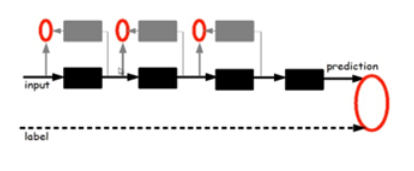
\includegraphics[width=0.5\textwidth]{pre-training}
\caption{pre-training}
%\label{fig:framework}
\end{figure}

\subsection{优化参数算法}
梯度下降(Gradient Descent,GD)是最小化风险函数、损失函数的一种常用方法,随机梯度下降和批量梯度下降时两种迭代求解思路,二者在一定程度上都可以优化参数。
\begin{itemize}
\item BSD(Batch Gradient Descent):批量梯度下降。~\\
也叫最速梯度下降法,它的求解思路如下:\\
\begin{enumerate}
\item 将J(theta)对theta求偏导,得到每个theta对应的的梯度:
\begin{displaymath}
\frac{\partial J(\theta)}{\partial {\theta_j}} =-\frac{1}{m}\sum_{i=1}^m(y^i-h_{\theta}(x^i))x^i_j
\end{displaymath}
\item 由于是要最小化风险函数,所以按每个参数theta的梯度负方向,来更新每个theta:
\begin{displaymath}
\theta_j=\theta_j+\frac{1}{m}\sum_{i=1}^m(y^i-h_{\theta}(x^i))x^i_j
\end{displaymath}
\item 从上面公式可以注意到,它得到的是一个全局最优解,但是每迭代一步,都要用到训练集所有的数据,如果m很大,那么这种方法的迭代速度会非常慢。
\end{enumerate}
\item SGD(Stochastic Gradient Descent):随机梯度下降。~\\
SGD是BSD的变种,使用SGD,将进行N次迭代,直到目标函数收敛,或者达某个既定的收敛界限。每次迭代都将对m个样本进行计算,计算量大,因此引入随机梯度下降法,他的求解思路如下:\\
\begin{enumerate}
\item 上面的风险函数可以写成如下这种形式,损失函数对应的是训练集中每个样本的粒度,而上面批量梯度下降对应的是所有的训练样本:
\begin{displaymath}
J(\theta)=\frac{1}{m}\sum_{i=1}^{m}\frac{1}{2}(y^i-h_{\theta}(x^i))^2=\frac{1}{m}\sum_{i=1}^{m}\cos t(\theta,(x^i,y^i))
\end{displaymath}
\begin{displaymath}
\cos t(\theta,(x^i,y^i))=\frac{1}{2}(y^i-h_{\theta}(x^i))^2
\end{displaymath}
\item 每个样本的损失函数,对theta求偏导得到对应梯度,来更新theta:
\begin{displaymath}
\theta_j=\theta_j+(y^i-h_{\theta}(x^i))^2{x^i_j}
\end{displaymath}
\item 随机梯度下降是通过每个样本来迭代更新一次,如果样本量很大的情况(例如几十万),那么可能只用其中几万条或者几千条的样本,就已经将theta迭代到最优解了,对比上面的批量梯度下降,迭代一次需要用到十几万训练样本,一次迭代不可能最优,如果迭代10次的话就需要遍历训练样本10次。但是,SGD伴随的一个问题是噪音较BGD要多,使得SGD并不是每次迭代都向着整体最优化方向。
\end{enumerate}
\end{itemize}

对二者的总结:

\begin{itemize}
\item 批量梯度下降---最小化所有训练样本的损失函数,使得最终求解的是全局的最优解,即求解的参数是使得风险函数最小。
\item 随机梯度下降---最小化每条样本的损失函数,虽然不是每次迭代得到的损失函数都向着全局最优方向, 但是大的整体的方向是向全局最优解的,最终的结果往往是在全局最优解附近。
\end{itemize}

\subsection{Batch-Normalization\cite{DBLP}}
批量归一化的算法是Google在论文《Batch Normalization: Accelerating Deep Network Training by Reducing Internal Covariate Shift》中提出来的,根据这个算法,如果我们对每一层的数据都进行处理,训练时间和overfit程度可以降低一些。 文中使用了类似z-score的归一化方式:每一维度减去自身均值,再除以自身标准差,由于使用的是随机梯度下降法,这些均值和方差也只能在当前迭代的batch中计算,故作者给这个算法命名为Batch Normalization。

Batch Normalization的加速作用体现在两个方面:一是归一化了每层和每维度的scale,所以可以整体使用一个较高的学习率,而不必像以前那样迁就小scale的维度;二是归一化后使得更多的权重分界面落在了数据中,降低了overfit的可能性,因此一些防止overfit但会降低速度的方法,例如dropout和权重衰减就可以不使用或者降低其权重。

\subsection{PReLU}
参数化修正线性单元PReLU, Parametric Rectified Linear Unit),是来自MRSA何恺明等研究员在论文《Delving Deep into Rectifiers: Surpassing Human-Level Performance on ImageNet Classification》中提出的。神经网络已经出现几十年了,大家都默认使用 Sigmoid/Tanh 函数作为非线性单元,直到近几年大家才意识到 ReLU 更好(更适合优化,精度也更好)。修正神经元 (rectifier neuron) 是近期将深度神经网络应用于计算机视觉挑战时取得成功的关键要素之一。这篇文章中提出了一种新的修正线性单元(ReLU, Rectified Linear Unit),并将其称为参数化修正线性单元(PReLU, Parametric Rectified Linear Unit)。

它的激活函数被定义为:
\begin{displaymath}
f(y_i) = max(0,y_i)+a_imin(0,y_i)
\end{displaymath}

其中 $a_i$ 是一个学习参数。下图是 ReLU 和 PReLU 的示意图:

\begin{figure}[!ht]
\centering
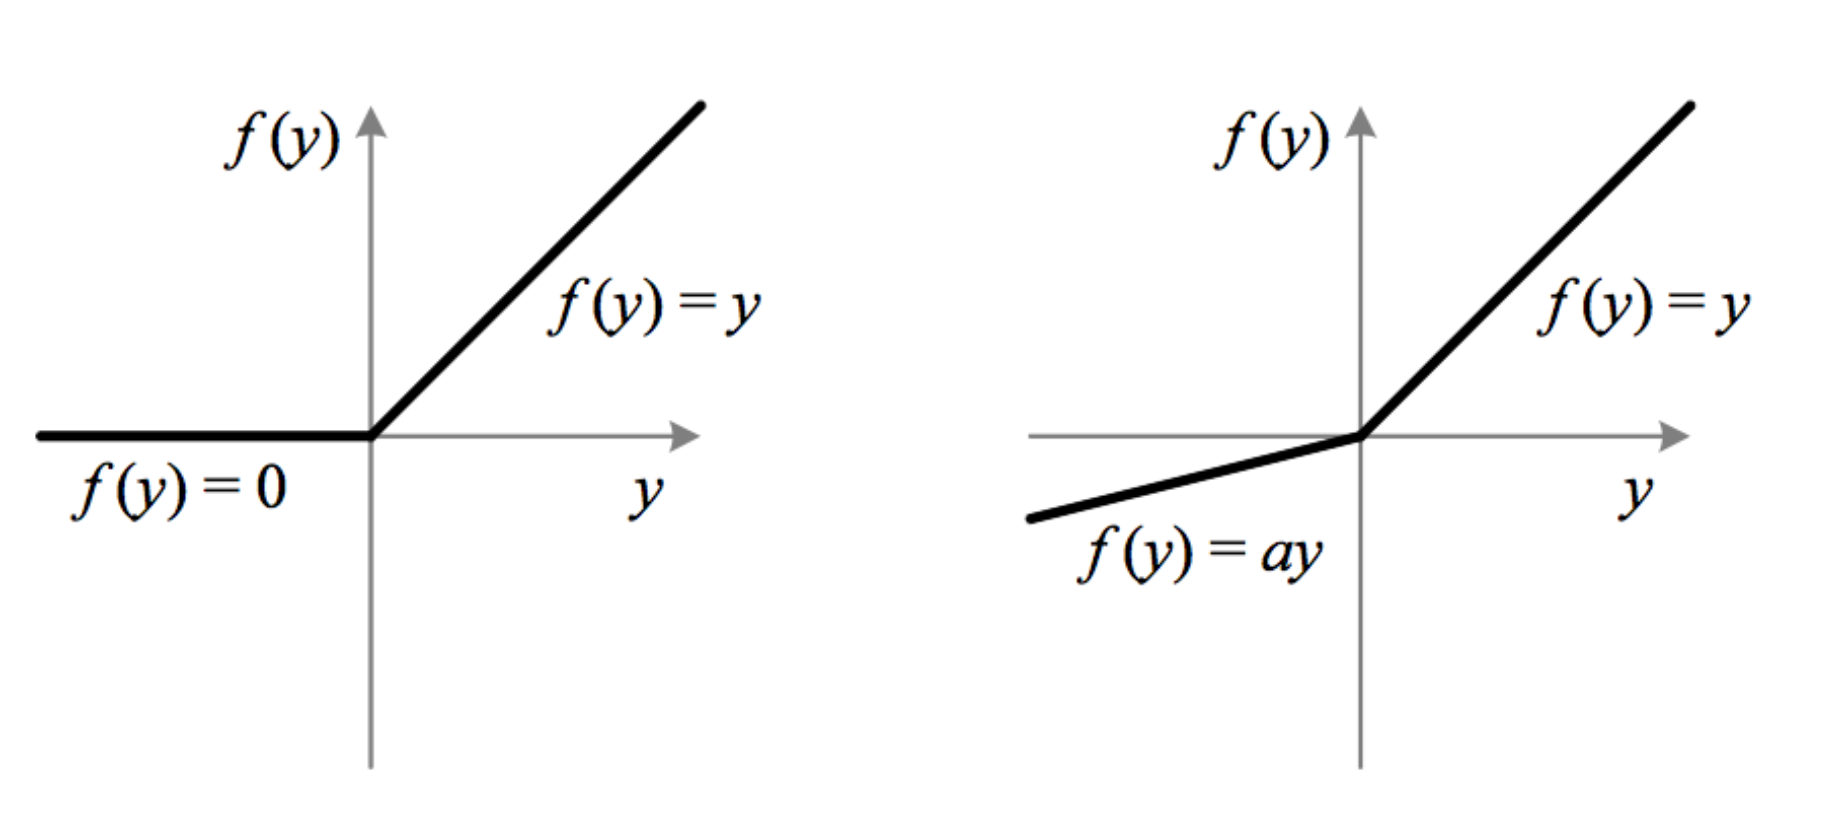
\includegraphics[width=0.5\textwidth]{PReLU}
\caption{ReLU 和 PReLU 的示意图}
%\label{fig:framework}
\end{figure}

该激活函数不仅可自适应获取修正参数,还可提高计算精度,且所需额外计算成本几乎可以忽略不计。

\section{解决方案}
\subsection{Caffe}
Caffe(Convolutional Architecture for Fast Feature Embedding)是纯粹的C++/CUDA架构,支持命令行、Python和MATLAB接口,且在CPU和GPU直接无缝切换。
\subsubsection{Caffe优点:}
\begin{itemize}
\item 上手快:模型与相应优化都是以文本形式而非代码形式给出。
\item 速度快:能够运行较好的模型与海量的数据。
\item 模块化:方便扩展到新的任务和设置上。
\item 开放性:公开的代码和参考模型用于再现。
\item 社区好:可以通过BSD-2参与开发与讨论。
\end{itemize}




\subsubsection{代码层次}
\begin{description}
\item[\textbf{Blob}] 基础的数据结构,{\color{blue} 保存学习到的参数}以及{\color{blue} 网络传输过程中产生数据的类}。\\
	主要是对protocol buffer所定义的数据结构的继承,Caffe也因此可以在尽可能小的内存占用下获得很高的效率。在更高一级的Layer中Blob用下面的形式表示学习到的参数:
	\begin{itemize}
	\item vector<sharedptr<Blob<Dtype> > > blob
	\item vector<Blob<Dtype>*> \& bottom
	\item vector<Blob<Dtype>*> *top
	\end{itemize}
\item[\textbf{Layer}] 网络的基本单元,由此派生出了各种层类。修改这部分的人主要是{\color{blue} 研究特征表达}方向的。\\
	用某种Layer来表示卷积操作,非线性变换,Pooling,权值连接等操作。具体分为5大类Layer:
	\begin{itemize}
	\item \textbf{NeuronLayer} \hspace{0.1in} 定义于neuron\_layers.hpp中,其派生类主要是元素级别的运算,运算均为同址计算。
	\item \textbf{LossLayer} \hspace{0.1in} 定义于loss\_layers.hpp中,其派生类会产生loss,只有这些层能够产生loss。
	\item \textbf{数据层} \hspace{0.1in} 定义于data\_layer.hpp中,作为网络的最底层,主要实现数据格式的转换。
	\item \textbf{特征表达层} \hspace{0.1in} 定义于vision\_layers.hpp,实现特征表达功能,例如卷积操作,Pooling操作等。
	\item \textbf{网络连接层和激活函数(待定)} \hspace{0.1in} 定义于common\_layers.hpp,Caffe提供了单个层与多个层的连接,并在这个头文件中声明。这里还包括了常用的全连接层InnerProductLayer类。
	\end{itemize}
	在Layer内部,数据主要有两种传递方式,\textbf{正向传导(Forward)}和\textbf{反向传导(Backward)}。Caffe中所有的Layer都要用这两种方法传递数据。
\item[\textbf{Net}] 网络的搭建,{\color{blue} 将Layer所派生出层类组合成网络}。\\
Net用容器的形式将多个Layer有序地放在一起,其自身实现的功能主要是对逐层Layer进行初始化,以及提供Update()的接口(更新网络参数),本身不能对参数进行有效地学习。
	\begin{itemize}
	\item vector<shared\_ptr<Layer<Dtype> > > layers \_
	\item vector<Blob<Dtype>*> \& Forward()
	\item void Net<Dtype>::Backward()
	\end{itemize}
\item[\textbf{Solver}] Net的求解,修改这部分人主要会是{\color{blue} 研究DL求解}方向的。\\
	这个类中包含一个Net的指针,主要是实现了训练模型参数所采用的优化算法,它所派生的类就可以对整个网络进行训练了。
	\begin{itemize}
	\item shared\_ptr<Net<Dtype> > net\_
	\item virtual void ComputeUpdateValue() = 0
	\end{itemize}
\end{description}

\subsection{CNN}
Deep Learning是全部深度学习算法的总称,CNN是深度学习算法在图像处理领域的一个应用。

\subsubsection{CNN优点:}
\begin{itemize}
\item 权值共享网络结构,降低网络模型的复杂度,减少了权值的数量。
\item 图像直接作为网络的输入,避免复杂的特征提取和数据重建。
\item 对平移、比例缩放、倾斜或者其他形式的变形具有高度不变性。
\end{itemize}

\subsubsection{CNN组成:}
\begin{itemize}
\item 局部感知
\item 参数共享
\item 多卷积核
\item Down-pooling
\item 多层卷积
\end{itemize}


\subsubsection{CNN网络配置文件:}
\begin{itemize}
\item Imagenet\_solver.prototxt (包含全局参数的配置文件)
\item Imagenet.prototxt (包含训练网络的配置文件)
\item Imagenet\_val.prototxt (包含测试网络的配置文件)
\end{itemize}



\subsection{AlexNet}
\subsubsection{网络结构}
AlexNet网络结构是CNN类型的DeepLearning网络模型在图像分类上的应用,如图Figure~\ref{fig:framework}。

\begin{figure}[!ht]
\centering
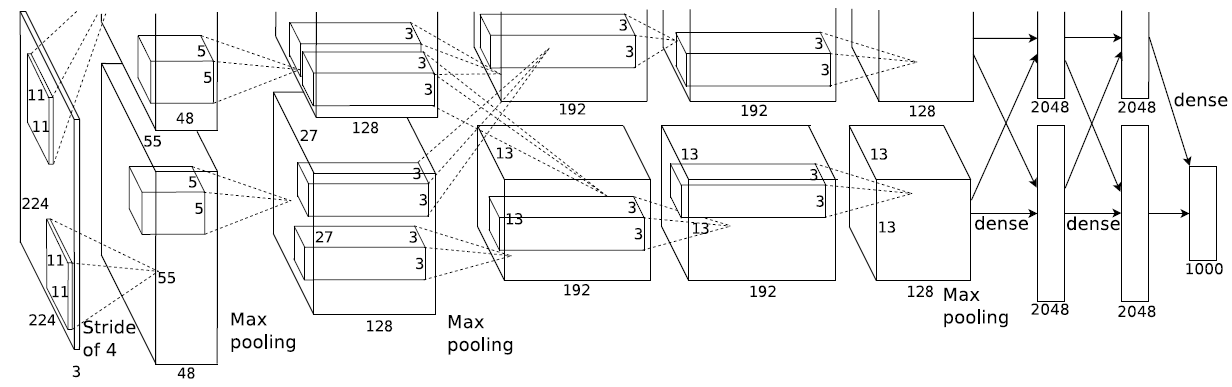
\includegraphics[width=0.8\textwidth]{AlexNet}
\caption{AlexNet}
\label{fig:framework}
\end{figure}

AlexNet网络模型训练了一个深度卷积神经网络,来将ILSVRC 2010中1.2M的高分辨率图像数据分为1000类。测试结果,Top-1和Top-5的错误率分别为37.5\%和17\%,优于当时最优的水平。后来作者修改了该模型参与了ILSVRC 2012竞赛,以Top-5错误率15.3\%遥遥领先亚军的26.2\%。

AlexNet网络模型用5个卷积层和3个全连接层,其中包含了60M参数和650K神经元。为使训练更快,AlexNet采用非饱和神经元,包括了大量不常见和新的特征来提升性能,减少训练时间。并利用了两个高效的GPU进行卷积运算。而这个层深度很重要,因为移除任何一个卷积层,将会导致更差的结果。网络大小主要受限于GPU的内存和训练时间。实验证明,本网络在有两个GTX 580 3GB GPU的机器上训练了5$\sim$6天。实验结果显示,如果GPU更快或数据集更大,实验结果将会更好。

%架构上的改进:
%	\begin{itemize}
%	\item ReLU非线性特征 
%	\item 在多GPU上训练
%	\item 局部响应标准化
%	\item 重叠采样
%	\end{itemize}
%\textbf{全局架构}:网络包括八个有权值的层。前五层是卷积层,剩下的三层是全连接层。其中,最后一个全连接层是输出层。第二、四、五个卷积层只与上层在同一个GPU上的Kernel Map(下文称特征图)连接,第三个卷积层与第二个卷积层的所有特征图连接。全连接层的神经元与上一层的所有神经元连接。响应标准化层在第一和第二个卷积层之后,降采样层在响应标准化层和第五个卷积层之后。而ReLU非线性公式在每个卷积层和全连接层都有应用。


为了简化实验,模型没有使用任何无监督学习。否则,在更大规模的网络和更长时间训练的情况下,AlexNet所得结果就能得到提高。另外,保持AlexNet网络模型的结构稳定,因为每移走一层中间的层,Top-1的错误率将会增高2\%。

\subsubsection{逐层功能实现:}
\begin{itemize}
\item 输入224$\times$224的图片,3通道
\item 第一层卷积 + pooling:11$\times$11的卷积核96个,步长为4,每个GPU各有48个。max-pooling的核为2$\times$2。如图Figure~\ref{fig:conv1}。
	\begin{figure}[!ht]
	\centering
	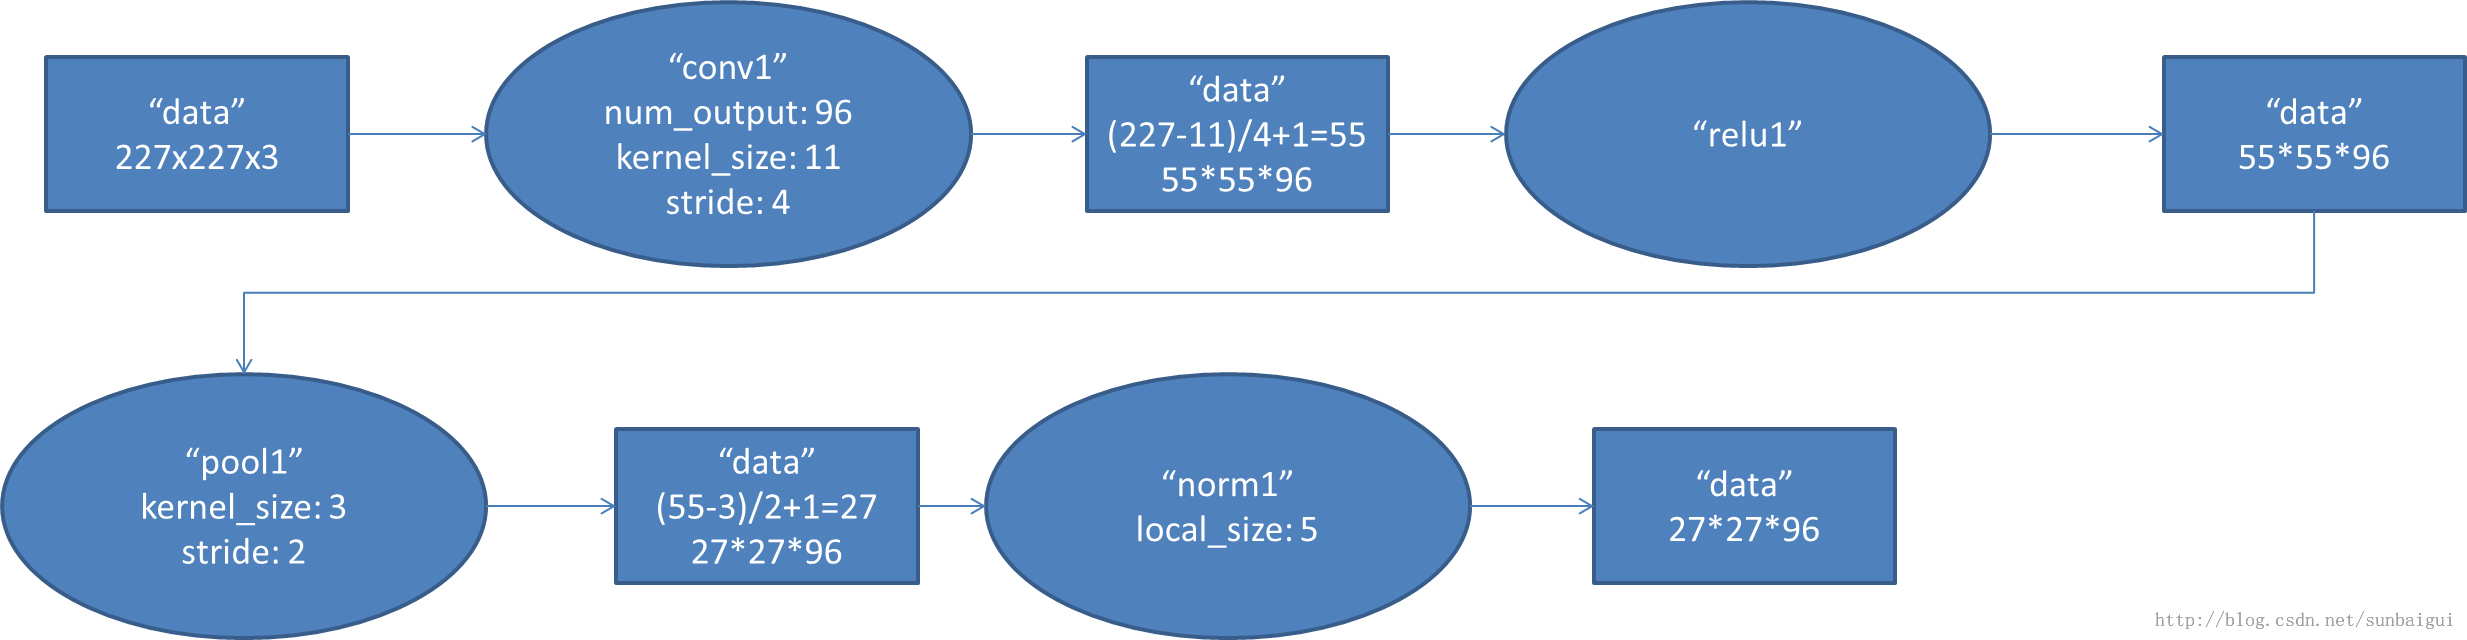
\includegraphics[width=0.7\textwidth]{conv1_1}
	\caption{Conv1}
	\label{fig:conv1}
	\end{figure}
\end{itemize}

\begin{itemize}
\item 第二层卷积 + pooling:5$\times$5的卷积核256个,每个GPU各有128个。max-pooling的核为2$\times$2。如图Figure~\ref{fig:conv2}。
	\begin{figure}[!ht]
	\centering
	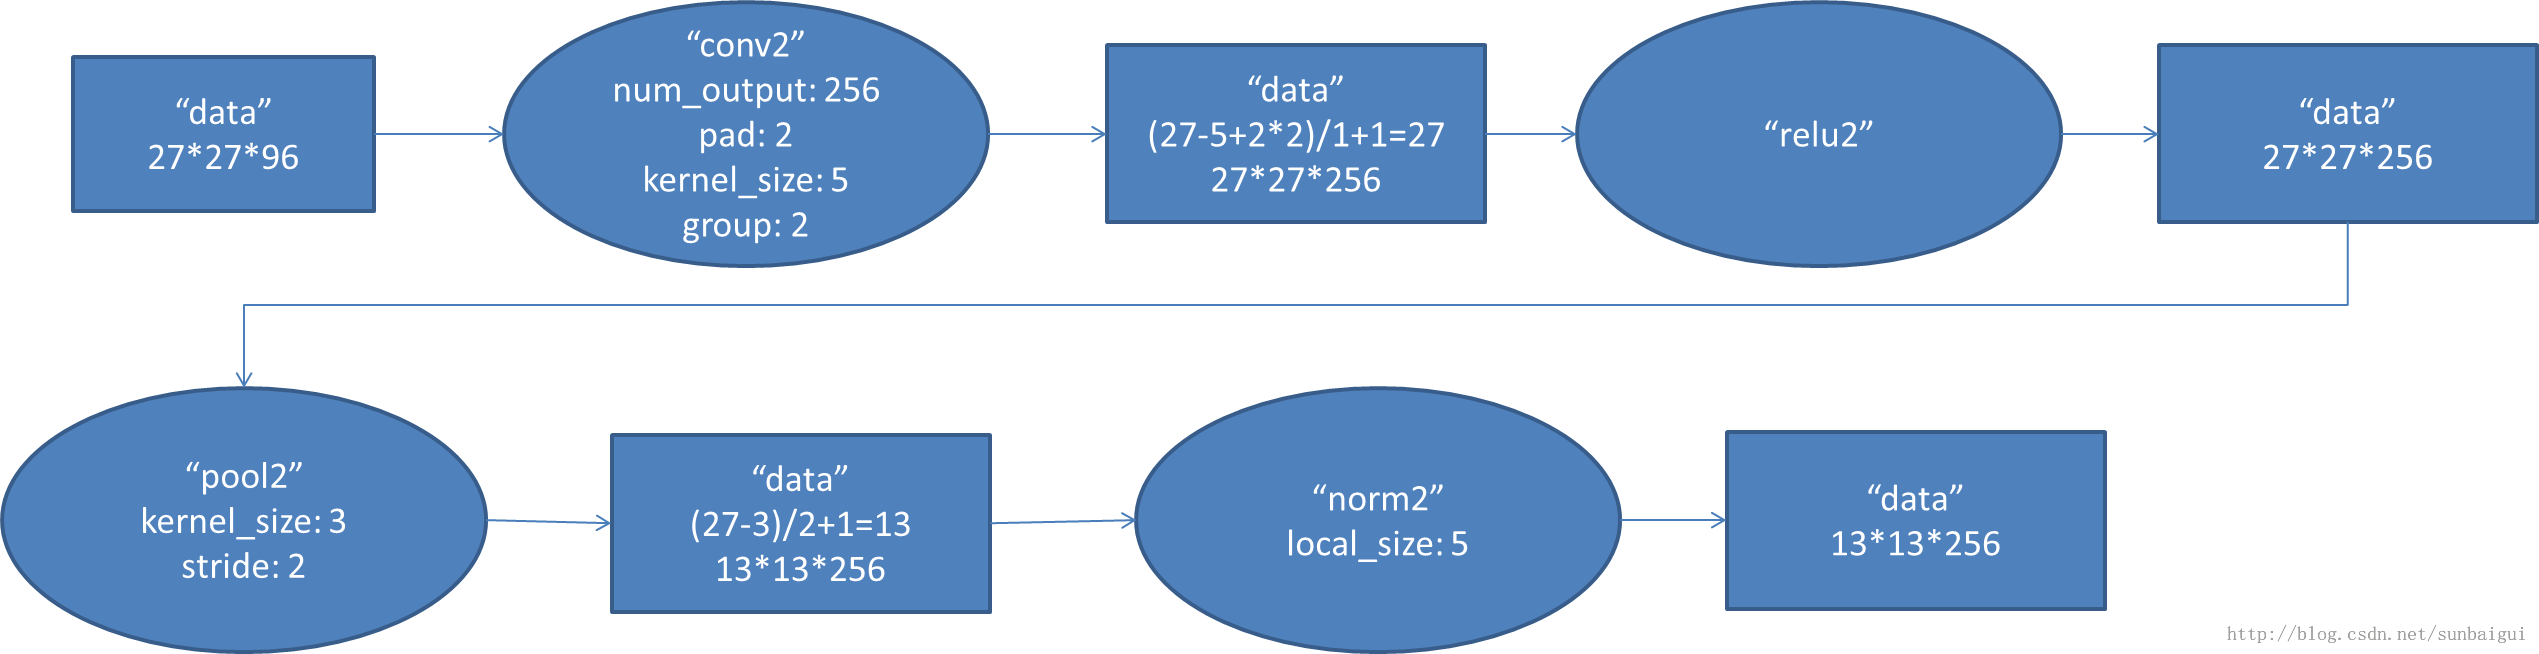
\includegraphics[width=0.7\textwidth]{conv2_2}
	\caption{Conv2}
	\label{fig:conv2}
	\end{figure}
\end{itemize}

\begin{itemize}
\item 第三层卷积:与上一层是全连接。3$\times$3的卷积核384个,每个GPU各有192个。如图Figure~\ref{fig:conv3}。
	\begin{figure}[!ht]
	\centering
	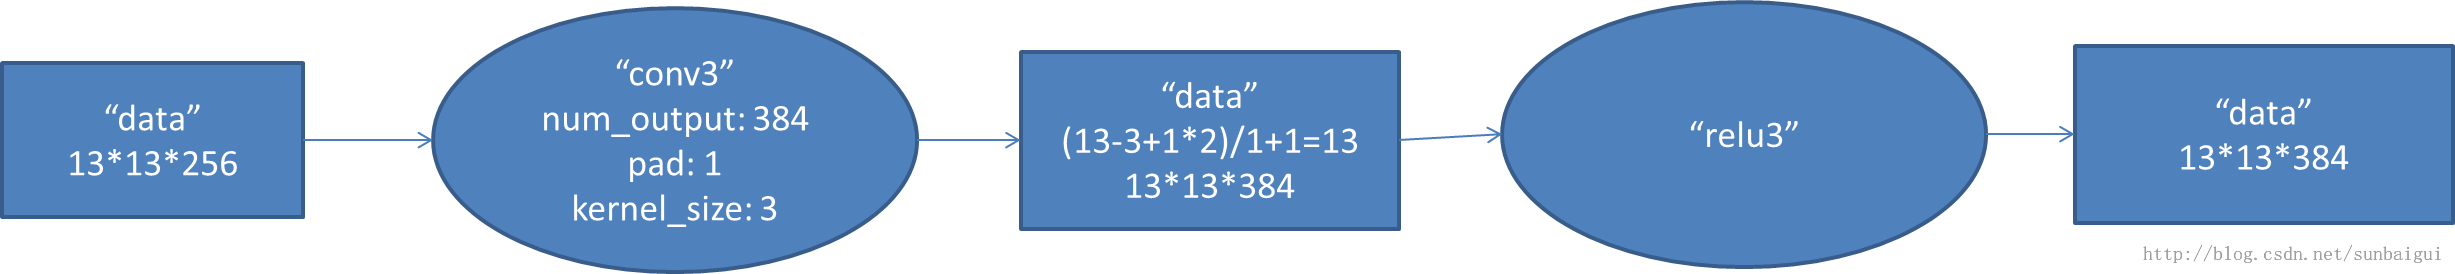
\includegraphics[width=0.7\textwidth]{conv3}
	\caption{Conv3}
	\label{fig:conv3}
	\end{figure}
\item 第四层卷积:3$\times$3的卷积核384个,每个GPU各有192个。如图Figure~\ref{fig:conv4}。
	\begin{figure}[!ht]
	\centering
	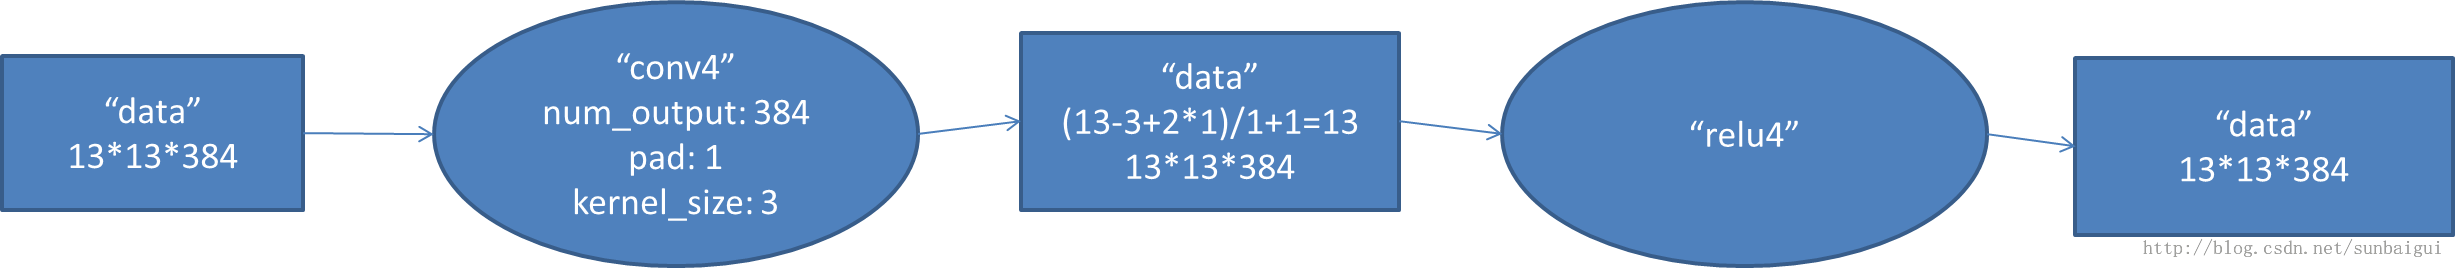
\includegraphics[width=0.7\textwidth]{conv4}
	\caption{Conv4}
	\label{fig:conv4}
	\end{figure}
\item 第五层卷积 + pooling:3$\times$3的卷积核256个,每个GPU各有128个。max-pooling:2 $\times$2的核。如图Figure~\ref{fig:conv5}。
	\begin{figure}[!ht]
	\centering
	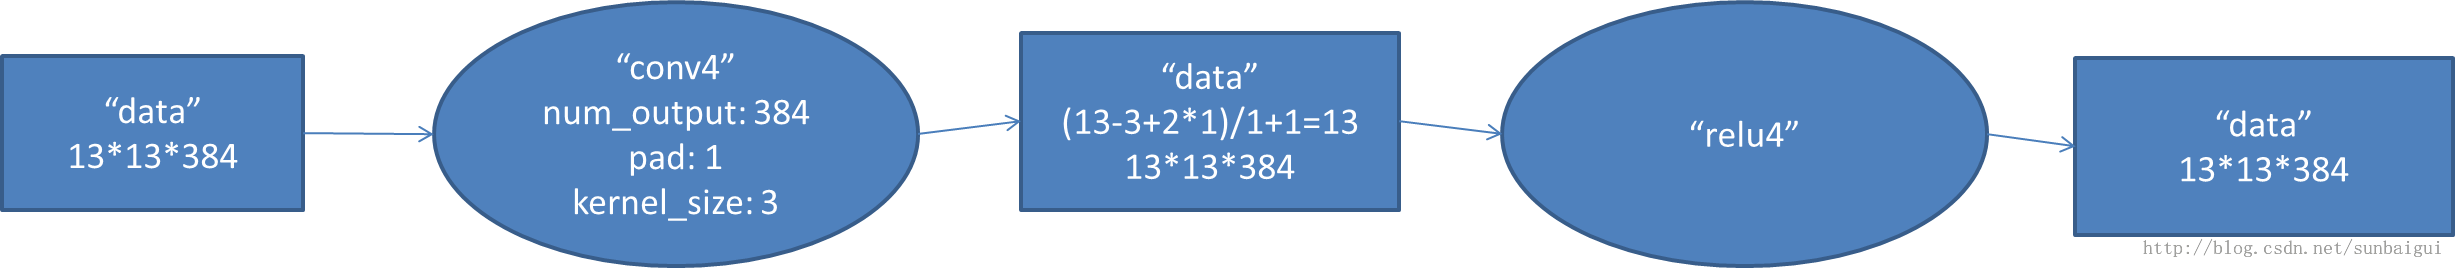
\includegraphics[width=0.7\textwidth]{conv4}
	\caption{Conv5}
	\label{fig:conv5}
	\end{figure}
\end{itemize}

\begin{itemize}
\item 第六层全连接:4096维,将第五层的输出连接成为一个一维向量,作为该层的输入。如图Figure~\ref{fig:fc6}。
	\begin{figure}[!ht]
	\centering
	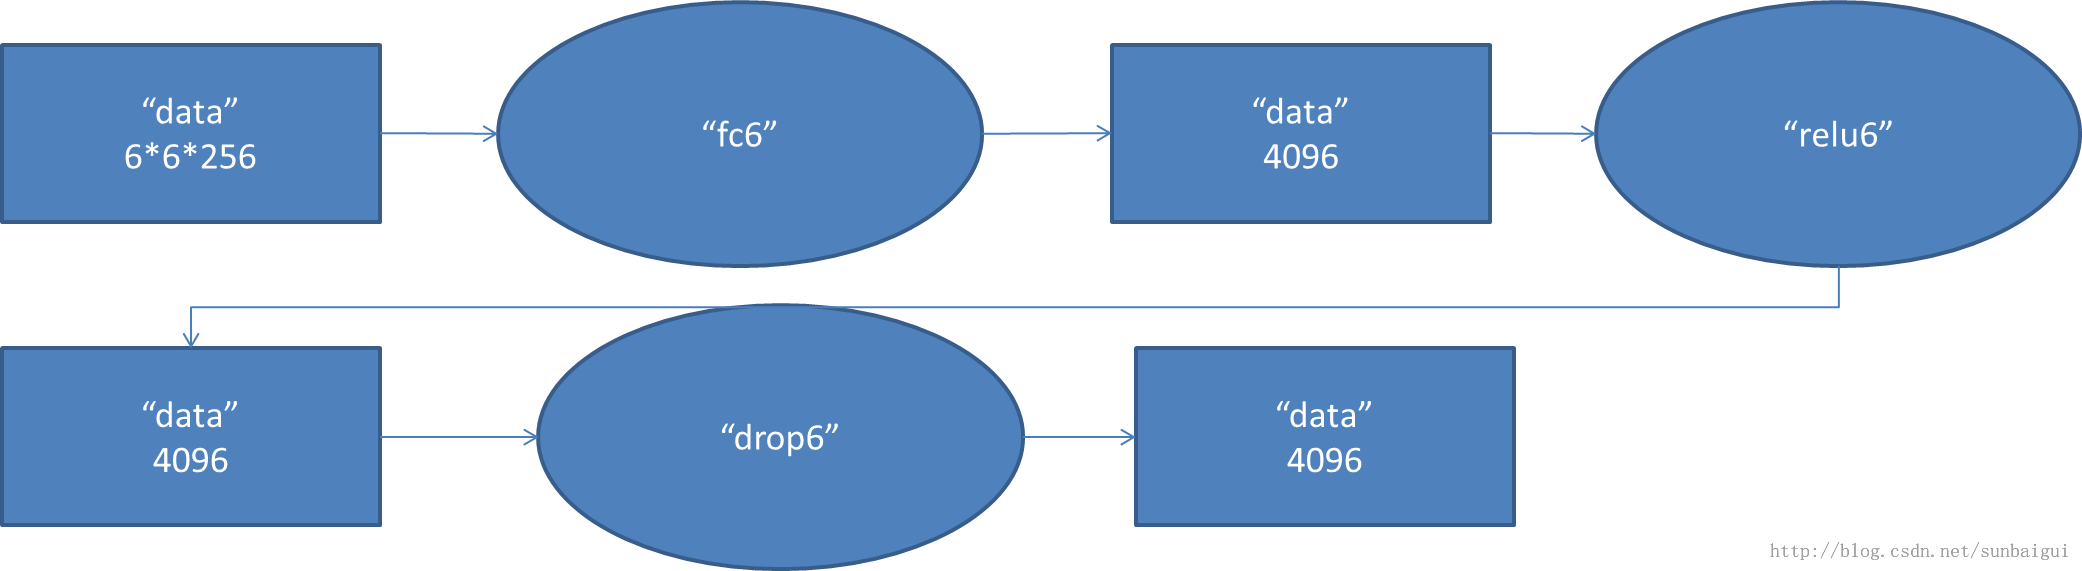
\includegraphics[width=0.5\textwidth]{fc1}
	\caption{Fc6}
	\label{fig:fc6}
	\end{figure}
\item 第七层全连接:4096维,将第六层的输出连接成为一个一维向量。如图Figure~\ref{fig:fc7}。
	\begin{figure}[!ht]
	\centering
	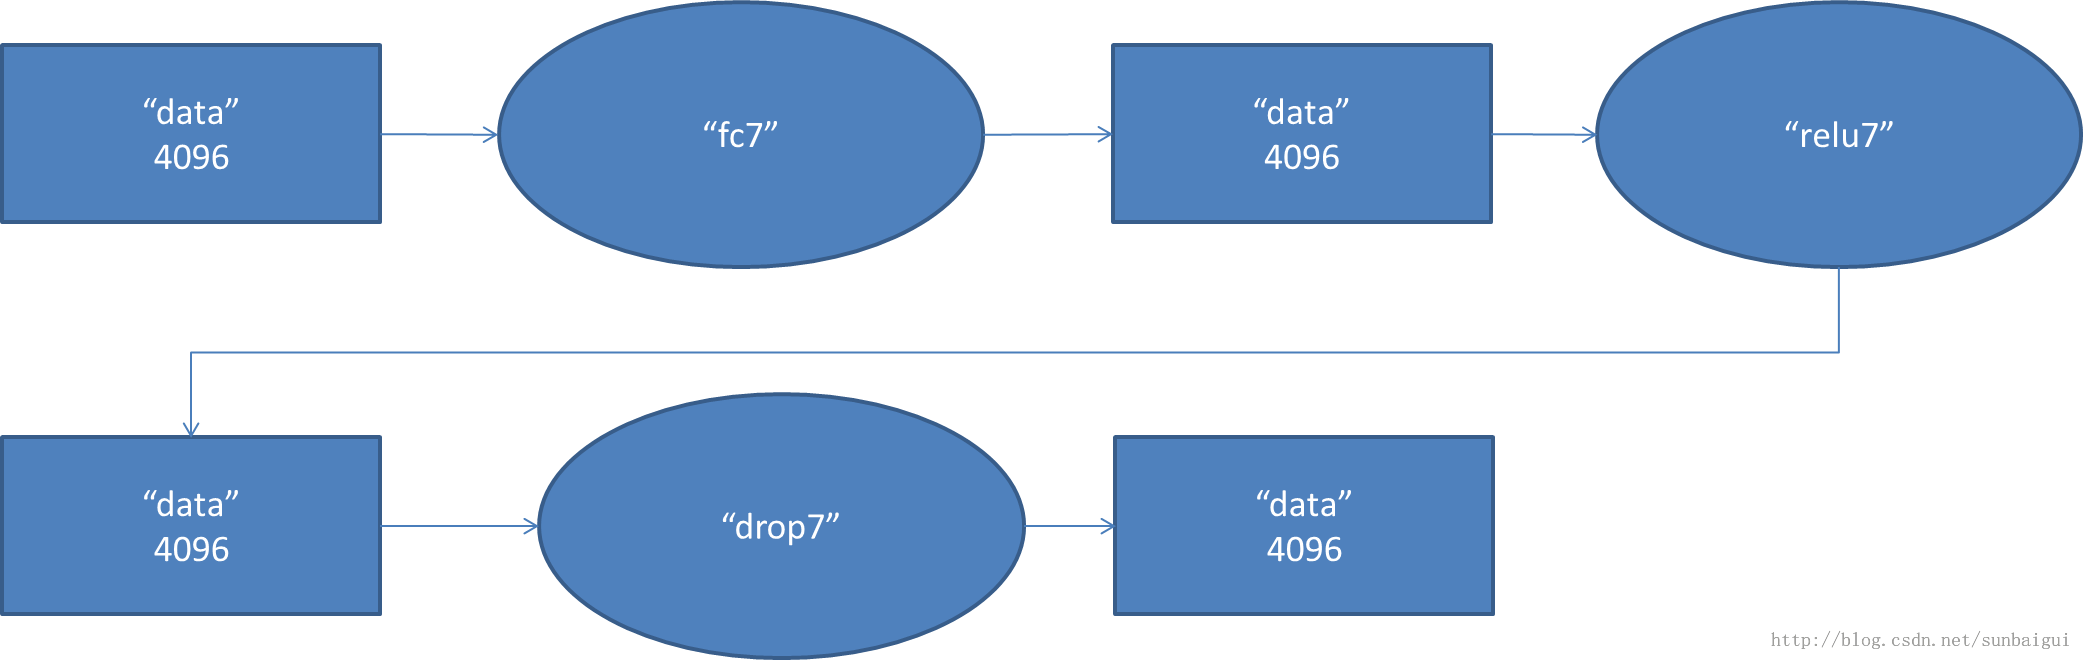
\includegraphics[width=0.5\textwidth]{fc2}
	\caption{Fc7}
	\label{fig:fc7}
	\end{figure}
\item Softmax层:输出为1000,输出的每一维都是图片属于该类别的概率。如图Figure~\ref{fig:fc8}。
	\begin{figure}[!ht]
	\centering
	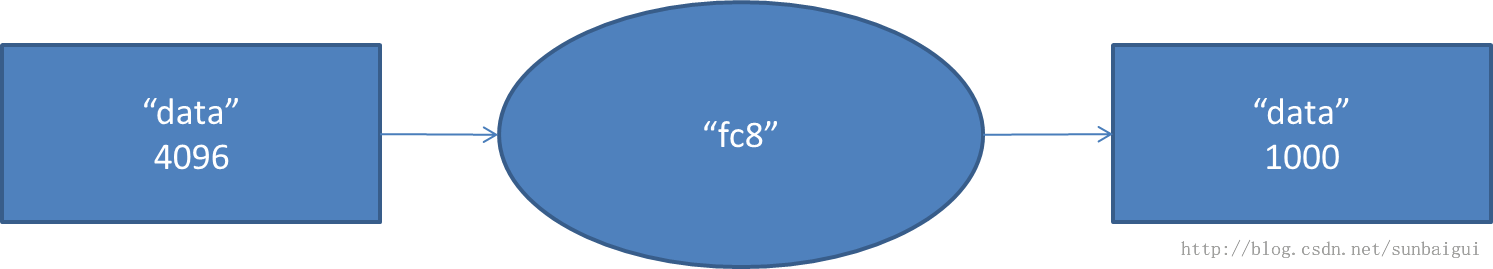
\includegraphics[width=0.5\textwidth]{fc3}
	\caption{Fc8}
	\label{fig:fc8}
	\end{figure}
\end{itemize}


\subsubsection{注意事项}
\begin{itemize}
\item 降低过拟合:
\begin{itemize}
\item 数据增强:通过提取图片的5个224*224切片(中间和四角)和它们的水平翻转来做出预测,预测结果为十次预测的平均值。第二种数据增强的方式为改变训练图像RGB通道的强度,对RGB空间做PCA,然后对主成分做高斯扰动。结果让错误率又下降了1\%。

\item Dropout:将某些层隐藏,按照50\%的概率输出0。这些隐藏的神经元不会参加CNN的forward过程,也不会参加back propagation过程。测试中,在前两个全连接层使用了该方法,使所有的神经元,但其输出都乘以0.5。如果没有dropout策略,AlexNet将会产生严重的过拟合。\newline
\end{itemize}

\item 架构上可改进方面:
\begin{itemize}
\item ReLU非线性特征 
\item 在多GPU上训练
\item 局部响应标准化
\item 重叠采样
\end{itemize}
\end{itemize}

\section{实施计划}

由于目前对于方案和优化技巧只是了解而已,因此我们决定不把大量的时间放在学习这些优化的算法上,我们准备从实际的问题入手,通过Caffe$+$AlexNet去做开发和实验,我们现在的问题在于确定训练集(跟老师讨论决定)。具体的计划暂定如下:

\begin{itemize}
\item 2015.07.06-2015.07.12
	
	完成第一次的训练集训练,并用训练好的特征进行分类,根据分类的效果确定改进方案。
\item 2015.07.13-2015.07.18

	根据改进方案完成第二次的训练,根据实际效果确认下一步的工作计划和方案
\end{itemize}



\bibliographystyle{plain}
\bibliography{ZooplanktonClassification_DL}

%%---------------------------------------------------------------------
\end{document}
